%!TEX root = linear-algebra.tex
\stepcounter{lecture}
\setcounter{lecture}{6}


\sektion{Angular Momentum}

\subsektion{Central Forces}
\lecturemarker{23}{22 Oct}
We will consider forces of the form
\[\vec{F} = F(r)\hat{r}\]
Magnitude depends on the distance from the origin. 

Direction $\hat{r}$ is repulsive; away from the origin. $-\hat{r}:$ attractive; towards the origin.\\ 

\begin{example}[Gravity]
\[\vec{F} = -\frac{GMm}{r^2}\hat{r}\]


\def\iangle{35} % Angle of the inclined plane

\def\down{-90}
\def\arcr{0.5cm} % Radius of the arc used to indicate angles

\begin{center}
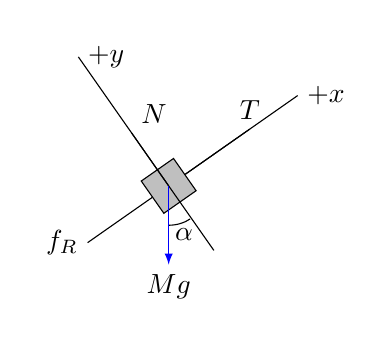
\begin{tikzpicture}[
    force/.style={>=latex,draw=blue,fill=blue},
    axis/.style={densely dashed,gray,font=\small},
    M/.style={rectangle,draw,fill=lightgray,minimum size=0.5cm,thin},
    m/.style={rectangle,draw=black,fill=lightgray,minimum size=0.3cm,thin},
    plane/.style={draw=black,fill=blue!10},
]

\matrix[column sep=1cm] {

    %% Free body diagram of M
    \begin{scope}[rotate=\iangle]
        \node[M,transform shape] (M) {};
        % Draw axes and help lines

        {[axis,->]
            \draw (0,-1) -- (0,2) node[right] {$+y$};
            \draw (M) -- ++(2,0) node[right] {$+x$};
            % Indicate angle. The code is a bit awkward.

            \draw[solid,shorten >=0.5pt] (\down-\iangle:\arcr)
                arc(\down-\iangle:\down:\arcr);
            \node at (\down-0.5*\iangle:1.3*\arcr) {$\alpha$};
        }

        % Forces
        {[force,->]
            % Assuming that Mg = 1. The normal force will therefore be cos(alpha)
            \draw (M.center) -- ++(0,{cos(\iangle)}) node[above right] {$N$};
            \draw (M.west) -- ++(-1,0) node[left] {$f_R$};
            \draw (M.east) -- ++(1,0) node[above] {$T$};
        }

    \end{scope}
    % Draw gravity force. The code is put outside the rotated
    % scope for simplicity. No need to do any angle calculations. 
    \draw[force,->] (M.center) -- ++(0,-1) node[below] {$Mg$};
    %%


\\
};
\end{tikzpicture}
\end{center}



\end{example}

Suppose that 

\def\iangle{35} % Angle of the inclined plane

\def\down{-90}
\def\arcr{0.5cm} % Radius of the arc used to indicate angles

\begin{center}
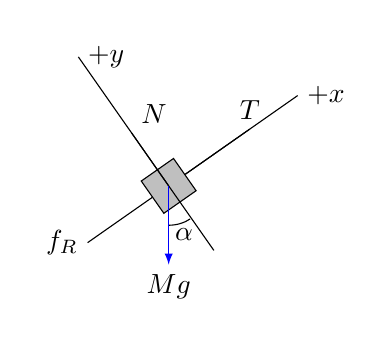
\begin{tikzpicture}[
    force/.style={>=latex,draw=blue,fill=blue},
    axis/.style={densely dashed,gray,font=\small},
    M/.style={rectangle,draw,fill=lightgray,minimum size=0.5cm,thin},
    m/.style={rectangle,draw=black,fill=lightgray,minimum size=0.3cm,thin},
    plane/.style={draw=black,fill=blue!10},
]

\matrix[column sep=1cm] {

    %% Free body diagram of M
    \begin{scope}[rotate=\iangle]
        \node[M,transform shape] (M) {};
        % Draw axes and help lines

        {[axis,->]
            \draw (0,-1) -- (0,2) node[right] {$+y$};
            \draw (M) -- ++(2,0) node[right] {$+x$};
            % Indicate angle. The code is a bit awkward.

            \draw[solid,shorten >=0.5pt] (\down-\iangle:\arcr)
                arc(\down-\iangle:\down:\arcr);
            \node at (\down-0.5*\iangle:1.3*\arcr) {$\alpha$};
        }

        % Forces
        {[force,->]
            % Assuming that Mg = 1. The normal force will therefore be cos(alpha)
            \draw (M.center) -- ++(0,{cos(\iangle)}) node[above right] {$N$};
            \draw (M.west) -- ++(-1,0) node[left] {$f_R$};
            \draw (M.east) -- ++(1,0) node[above] {$T$};
        }

    \end{scope}
    % Draw gravity force. The code is put outside the rotated
    % scope for simplicity. No need to do any angle calculations. 
    \draw[force,->] (M.center) -- ++(0,-1) node[below] {$Mg$};
    %%

\\
};
\end{tikzpicture}
\end{center}



Polar coordinates are perfect for these problems

Newton's Second Law:
\begin{equation}m(\ddot{r}-r\dot{\theta}^2) = F\end{equation}
\vspace*{-10pt}
\begin{equation}m(r\ddot{\theta} + 2\dot{r}\dot{\theta}) = 0\end{equation}

Multiply (6.3) by $r$
\[m(r^2\ddot{\theta} + 2\dot{r}r\dot{\theta}) = 0\]
\[\frac{d}{dt}(mr^2\dot{\theta}) = 0 \implies mr^2\dot{\theta} = mh = \text{constant}\]
\begin{definition}
$h = r^2\dot{\theta}$ - \emph{angular momentum per unit mass}

\emph{Angular momentum}, $\vec{J} = \vec{r} \times \vec{p} = \vec{r} \times m \vec{v}$
\end{definition}
\begin{theorem}[Conservation of Angular Momentum]
	Under a central force (no torque), the total angular momentum is conserved.
\end{theorem}

\begin{proof}
In polars, $\vec{r} = r\hat{r}$,~$\vec{v} = \dot{r}\hat{r} + r\dot{\theta}\hat{\theta}$
\[\vec{J} = \vec{r} \times m\vec{v} = (r\hat{r}) \times m(\dot{r}\hat{r} + r\dot{\theta}\hat{\theta}) = mr\dot{r}(\hat{r}\times\hat{r}) + mr^2\dot{\theta}(\hat{r} \times \hat{\theta}) \]
\[\implies \vec{J} =  mr^2\dot{\theta}\hat{k} = mh\hat{k} = \text{ constant }\qedhere\]
\end{proof}


\subsubsektion{Energy}

For a force to be conservative $\vec{F} = -\vec{\nabla}V$. In 2D

\begin{equation}\vec{F} = -\frac{\partial V}{\partial x}\hat{i} - \frac{\partial V}{\partial y}\hat{j}\end{equation}
Since $\vec{F} = \vec{F}(r)\hat{r}$ we need $V = V(r)$
\[\frac{\partial V}{\partial x} = \frac{dV}{dr}\frac{\partial r}{\partial x}\]
Since $r = (x^2 + y^2)^{1/2}$, $\dfrac{\partial r}{\partial x} = \frac{1}{2}[x^2 + y^2]^{1/2}\times(2x) = x/r = \cos(\theta)$.
Thus 
\[\frac{\partial V}{\partial x} = \frac{dV}{dr}\cos\theta\]

Similarly \[\frac{\partial V}{\partial y} = \frac{dV}{dr}\frac{\partial r}{\partial y} = \frac{dV}{dr}\sin\theta\]~\\

Thus the force, by (6.5), is
\[\begin{aligned}\vec{F} &= -\frac{dV}{dx}\cos\theta\hat{i} - \frac{dV}{dy}\sin\theta\hat{j}\\
 &= -\frac{dV}{dr}\hat{r}
\end{aligned}
\]

So for a central force to be conservative
\[\vec{F}(r) = -\frac{dV}{dr}\]

From the Conservation of Energy
\[\frac{1}{2}mv^2 + V(r) = E\]
Since $\vec{v} = \dot{r}\hat{r} + r\dot{\theta}\hat{\theta}$
\begin{equation}\boxed{E = \frac{1}{2}m[\dot{r}^2 + r^2\dot{\theta}^2] + V(r)}\end{equation}
\pagebreak


\subsektion{Orbital Equation}
Find the trajectories or shapes or orbits as a function of $\theta$. It's solution is $u(\theta) = 1/r(\theta)$. 


We know $h = r^2\dot{\theta} = \dot{\theta}u^{-2} \implies \dot{\theta} = hu^2$. Thus
\[\dot{r} = \frac{d}{dt}(u^{-1}) = -u^{-2}\frac{du}{d\theta}\frac{d\theta}{dt} = -h\frac{du}{d\theta}\]
\[\ddot{r} = -h\frac{d}{dt}\left(\frac{du}{d\theta}\right) = -h\frac{d^2u}{d\theta^2}\dot{\theta} = h^2u^2\frac{d^2u}{d\theta^2}\]
Also 
\[r\dot{\theta}^2 = u^{-1}(hu^2)^2 = h^2u^3\]


Write $F(r) = F(u^{-1})$ and substitute into (6.2) from Newton's 2nd Law:
\[m(h^2u^2\frac{d^2u}{d\theta^2} - h^2u^3) = F(u^{-1})\]
Giving our orbital equation:
\begin{equation} \boxed{\frac{d^2u}{d\theta^2} + u = -\frac{1}{mh^2u^2}F(u^{-1})} \end{equation}~

\begin{example}
	$r(\theta) = c\theta^2 ~(c > 0)$. Find $F(r)$:
	\[u = c^{-1}\theta^{-2},~\dfrac{du}{d\theta} = -2c^{-1}\theta^{-3},~\dfrac{d^2u}{d\theta^2} = 6c^{-1}\theta^{-4} = 6u^2\]
	
	From the Orbital Equation (6.6)
	\[F(u^{-1}) = -mh^2u^2(u + 6cu^2) = -mh^2(u^3 + 6cu^4)\]
	\[\implies F(r) = -mh^2(r^{-3} + 6cr^{-4})\] 
\end{example}



\subsubsektion{Kepler's Laws}
\lecturemarker{24}{22 Oct}

\begin{theorem}[Kepler's Laws]
	\begin{enumerate}
	\item[I] Orbits of Planets are Ellipses	
	\item[II]Law of Equal Areas: If $\Delta t_1 = \Delta t_2$ then $A_1 = A_2$

	\item[III] The time period of orbit, $T \propto a^3$
	
	\begin{center}
	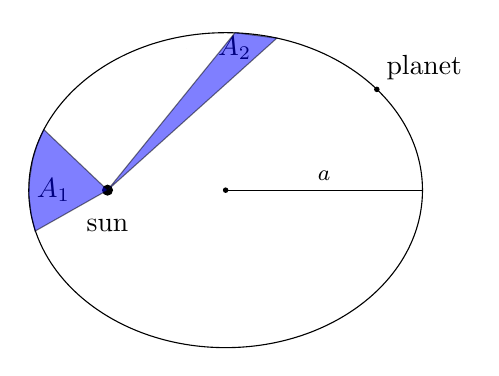
\begin{tikzpicture}
      \draw [rotate around={0:(1.5,0)}] (1.5,0) ellipse (2.5cm and 2cm);
%
      \fill (0,0) coordinate (O) circle (2pt) node[below =7pt] {sun};
      \fill (0,0) coordinate (O) circle (0pt) node[left =10pt] {$A_1$};
      \fill (1,1.8) coordinate (blah) circle (0pt) node[right =8pt] {$A_2$};
      %
      \coordinate (A1) at (1.62,2) ;%%
      \coordinate (A2) at (2.15,1.93);%%
      \coordinate (B1) at (-0.81,0.77);%%
      \coordinate (B2) at (-0.9,0.56);%%
      \coordinate (B3) at (-0.95,0.39);%%
      \coordinate (B4) at (-0.99,0.14);%%
      \coordinate (B5) at (-1,-0.05);%%
      \coordinate (B6) at (-0.97,-0.31);%%
      \coordinate (B7) at (-0.92,-0.52);%%
    %
%
      \coordinate (C1) at (3.25,-1.43);%%
      \coordinate (C2) at (3.51,-1.18);%%
%
      \coordinate (P) at (3.42,1.28) ;%%
      \fill (P) circle (1pt) node[above right] {planet};%
%
%
      \filldraw[fill=blue,opacity=0.5] (O) -- (A1) -- (A2) --cycle;%
      \filldraw[fill=blue,opacity=0.5] (O) -- (B1) -- (B2) -- (B3) -- (B4) -- (B5) -- (B6) -- (B7)
      --cycle;%
%

      \draw (1.5,0) coordinate (M) --node[above]{\footnotesize $a$}
      (4,0);%
      
      \fill (M) circle (1pt);
   \end{tikzpicture}
	\vspace*{-4pt}
	\end{center}


	\end{enumerate}

\end{theorem}



\begin{proof}[Proof of Kepler's First Law]
Inverse square law:
\[F(r) = -k/r^2 \implies F(u^{-1}) = -ku^2\]
Substituting into our orbital equation (6.6)
\[\frac{d^2u}{d\theta^2} + u = \frac{k}{mh^2u^2} ~(*)\]

This resembles \[m\frac{d^2x}{dt^2} + kx = F_0\]
The general solution to $(*)$ is $u = A\cos(\theta-\theta_0) + \dfrac{k}{mh^2}$;
 wlog take $\theta_0 = 0$ so
\[u(\theta) = A\cos(\theta) + \dfrac{k}{mh^2}\]
\begin{equation}\implies r(\theta) = \frac{(mh^2/k)}{1 + \frac{Amh^2}{k}\cos\theta}\end{equation}


This is the form of an ellipse in polar coordinates (see Problem 10, P.S. 1)
 
\[r(\theta) = \frac{l}{1 + e\cos\theta}\]
Where $l = \dfrac{mh^2}{k}$, $e = \dfrac{Amh^2}{k}$. \vspace*{150pt}

$e = [1-b^2/a^2]^{1/2}$,~$l = a(1-e^2)$ \end{proof}

We see that $E$ is related to $A$.
 
We can get the family of orbits by considering the energy; equation (6.5) gives
\[E = \frac{1}{2}m[\dot{r}^2 + r^2\dot{\theta}^2] + V(r)\]
 
 
 $F(r) =-kr^{-2} = -\dfrac{dV}{dr}$, so $ V(r) = -kr^{-1} \implies V(u^{-1}) = -ku$. 

Also $\dot{r} = -h\dfrac{du}{d\theta}$, and $r^2\dot{\theta}^2 = h^2r^{-2} = h^2u^2$. So the energy is
\[E = \frac{1}{2}mh^2\left[\left(\frac{du}{d\theta}\right)^2 + u^2\right]-ku\]
Using the fact $u(\theta) = A\cos(\theta) + \dfrac{k}{mh^2}$, $\dfrac{du}{d\theta} = -A\sin\theta$ and simplifying the trig we get
\[E = \frac{1}{2}mh^2A^2 - \frac{1}{2}\frac{k^2}{mh^2}\]
\[\implies A = \sqrt{\frac{2E}{mh^2} + \frac{k^2}{(mh^2)^2} }\]


From (6.9), the eccentricity of the orbit, $e = (1-b^2/a^2)^{1/2}$, is
\[e = \frac{Amh^2}{k} = \frac{mh^2}{k}\sqrt{\frac{2E}{mh^2} + \frac{k^2}{(mh^2)^2} } = \sqrt{1 + \frac{2Emh^2}{k^2}}\]
	

This parameter $e$ actually allows our solution $r(\theta)$ to describe a whole family of orbits. 
\begin{examples}
\begin{enumerate}
\item Bounded Trajectories
\begin{itemize}
\item $E = -k^2/2mh^2 \implies e = 0$ [Circle] 	
\item $E < 0 \implies 0 < e < 1$ [Ellipse]
\end{itemize}

\item Unbounded Trajectories
\begin{itemize}
\item $E = 0 \implies e = 1$ [Parabola]
\item $E > 0 \implies e > 1$ [Hyperbola]	
\end{itemize}

\end{enumerate}
	
\end{examples}

\subsektion{Effective Potential}
\lecturemarker{25}{22 Oct}
Consider the energy 
\[E = \frac{1}{2}m\dot{r}^2 + \frac{1}{2}mr^2\dot{\theta}^2 + V(r)\]

Since $h = r^2\dot{\theta},~ h^2 = r^4\dot{\theta}^2 \implies r^2\dot{\theta}^2 = h^2/r^2$
\[E = \frac{1}{2}m\dot{r}^2 + \frac{1}{2}\frac{mh^2}{r^2} + V(r)\]

\begin{definition}
The \emph{Effective Potential}, $V_{EFF} =\dfrac{1}{2}\dfrac{mh^2}{r^2} + V(r)$	
\end{definition}
\[\implies E = \frac{1}{2}m\dot{r}^2 + V_{EFF}\]
What we've done is written our energy in such a way that it looks like what we had with 1D motion! 
\[\begin{aligned}x &\longrightarrow r \\
V(x) &\longrightarrow V_{EFF}(r)
\end{aligned}
\]

\begin{definition} \emph{Turning points} occur when $V_{EFF} = E$. This tells us where $\frac{1}{2}m\dot{r}^2 = 0 \implies \dot{r} = 0$. This tells us about the boundedness of our orbit. 

\end{definition}
\pagebreak

\subsubsektion{Equilibria}
In 1D: $V'(x_0) = 0 \implies F(x_0) = 0$, where $x_0$ is the equilibrium point

If $\dot{x} = 0$ and $x = x_0$ at $t = 0$, then $m\ddot{x} = 0$ and $x = x_0~\forall t$

\[V_{EFF} =\dfrac{1}{2}\dfrac{mh^2}{r^2} + V(r)\]
\[\implies \frac{dV_{EFF}}{dr} = -mh^2r^{-3} + \underbrace{V'(r)}_{-F(r)}\]

Newton's 2nd Law's $\hat{r}$ component (equation (6.2))
\[m(\ddot{r} - r\dot{\theta}^2) = F(r)\]
\[\implies m\ddot{r} = F(r) + \frac{mh^2}{r^3} = \frac{dV_{EFF}}{dr}\]

Suppose that $V'_{EFF}(r_0) = 0$. If $r = r_0$ and $\dot{r} = 0$ at $t = 0$, then $m\ddot{r} = 0 \implies r = r_0~\forall t$. So we have a constant $r\implies $ Circular Trajectory

\subsubsektion{Stability}
$R = r-r_0$, $|R| << 1$, then the Taylor expansion about $r_0$:
\begin{equation}V_{EFF}(r) = V_{EFF}(r_0) + RV'_{EFF}(r_0) + \frac{1}{2}R^2V''_{EFF}(r_0) + \dots	
\end{equation}


Since at $r_0$, $V'_{EFF}(r_0) = 0$
\[V_{EFF}(r) = V_{EFF}(r_0) + \frac{1}{2}R^2V''_{EFF}(r_0)\]
Differentiating
\[V'_{EFF}(r) = RV''_{EFF}(r)\]

Using this in Newton's Second Law: 
\[m\ddot{r} = -RV''_{EFF}(r_0)\]
or 
\[m\ddot{R} + RV''_{EFF}(r_0)= 0\]

\begin{itemize}
\item If $V''_{EFF}(r_0)>0 \implies$ a minimum, so the circular orbit is stable.

\item If $V''_{EFF}(r_0) < 0 \implies$ a maximum, so the circular orbit is unstable. 
\end{itemize}~


\begin{example}
	$F(r) = -kr^{-2} ~(k > 0) \implies V(r) = -kr^{-1}$
	
	 \[\implies V_{EFF}(r) = -kr^{-1} + \frac{1}{2}mh^2r^{-2}\] 
	 \[\implies V'_{EFF}(r) = kr^{-2} - mh^2r^{-3}\]
	 
	 Setting this equal to zero 
	 \[r^{-3}(kr -mh^2) = 0\]
	 This is satisfied as $r \to \infty$ or at $r_0 = mh^2/k$
	 
	 \[V''_{EFF}(r) = -2kr^{-3} + 3mh^2r^{-4}\]
	 
	 So at the equilibria point
	 \[V''_{EFF}(mh^2/k) = \left(\frac{k}{mh^2}\right)^4(3mh^2 - 2k(mh^2/k)) = \left(\frac{k}{mh^2}\right)^4(mh^2)  > 0\]
	 This is a stable circular trajectory.
	 
	 \vspace*{150pt}
	 
\[ V'_{EFF}(\frac{mh^2}{k}) = -k\left(\frac{k}{mh^2}\right) + \frac{1}{2}mh^2\left(\frac{k^2}{(mh^2)^2}\right) = -\frac{k^2}{2mh^2}\] 

Thus \[E_{MIN} = -\frac{k^2}{2mh^2}.\]


We reach the same family of orbits as Example 6.10 by differing values of $E$:
\begin{enumerate}
\item Bounded Trajectories
\begin{itemize}
\item $E = E_{MIN} = -k^2/2mh^2 \implies r = \frac{mh^2}{k} \implies$ Circular Orbit
\item $E_{MIN} < E < 0 \implies $ two turning points $\implies$ Bounded Orbit [Ellipse]

\end{itemize}

\item Unbounded Trajectories when $E \geq 0$ since we have only a single turning point. In particular
\begin{itemize}
\item $E = 0 \implies $ Parabola
\item $E > 0 \implies $ Hyperbola
\end{itemize}

\end{enumerate}
\end{example}



